\documentclass[12pt]{article}

\usepackage{xeCJK}%字體設定
\setCJKmainfont{cwTeXKai}[AutoFakeBold=1.5]


\setmainfont{Times New Roman}  % 英文正文字體

\usepackage[top=2cm,bottom=2cm,left=2cm,right=2cm,a4paper]{geometry}%版面設定

\usepackage{indentfirst}%縮排

\usepackage{setspace}%行距設計
\onehalfspacing%半行距
\setlength{\parskip}{3pt}%段落之間

\usepackage{moresize}%字體大小

\usepackage{graphicx}

\usepackage{amssymb}%數學符號

\usepackage{amsmath} % 數學符號
\usepackage{booktabs}         % 漂亮的表格（\toprule, \midrule, \bottomrule）
\usepackage{siunitx}          % 國際單位制 (建議處理單位更漂亮)

\usepackage{multicol}%引入函數使下面那些可以變成雙欄

\usepackage{float}%圖片固定

\usepackage{gensymb}

% \renewcommand{\thesection}{\Roman{section}}


%%%%%%%%%%%%%%%%%%%%%%%%%%%%%%正文%%%%%%%%%%%%%%%%%%%%%%%%%%%%%%%%%%%
\begin{document}

\begin{titlepage}
\begin{center}

\vspace*{0.5cm}
\HUGE \textbf{普通物理實驗結報}\\
\vspace{1cm}
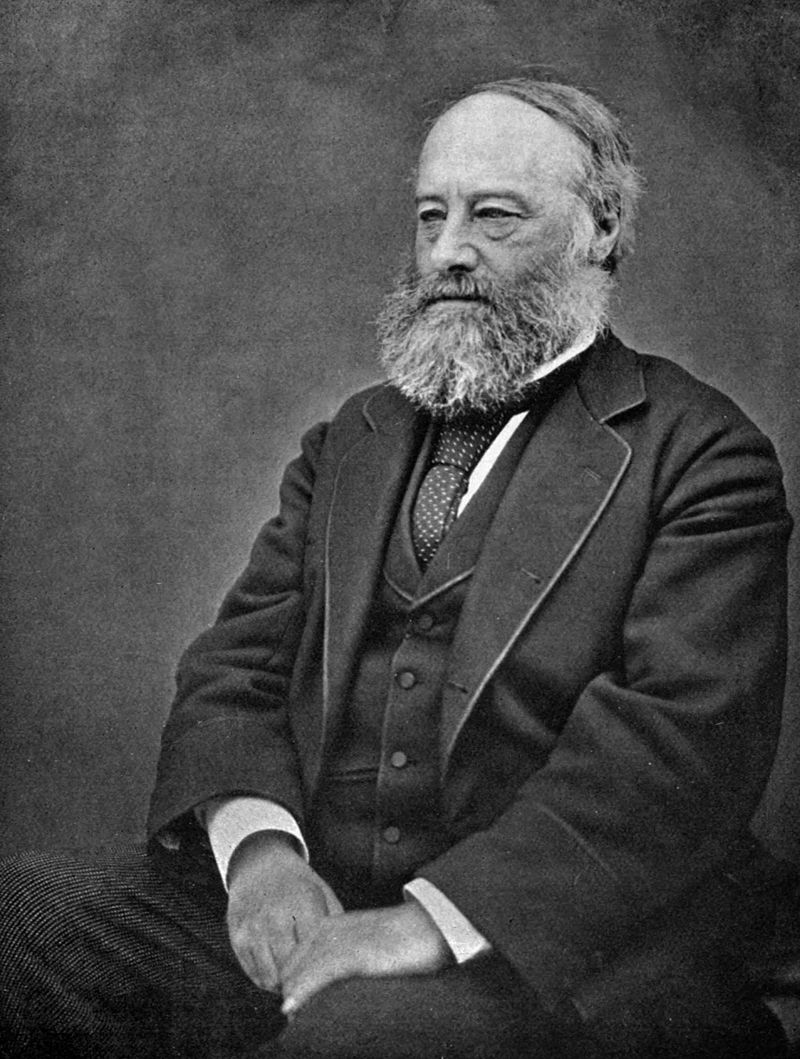
\includegraphics[width=9cm]{熱功當量/nBnaugDOxEWOmhDZmBTM1MGNkFjNiNjN5IGZzMzMjBDM2ImN0IjNmNjNhZzLtVGdp9yYpB3LltWahJ2Lt92YuUHZpFmYuMmczdWbp9yL6MHc0RHa.jpg}\\[2cm]
\HUGE \textbf{熱功當量}\\

\vfill
\huge 第三組\\[0.5cm]
\begin{table}[h]
\centering
\Large
\begin{tabular}{|c|c|}
\hline
組員:              & 貢獻度  \\
吳& 35\% \\
卓& 35\% \\
程& 30\% \\ \hline
\end{tabular}
\end{table}

\end{center}

\end{titlepage}

%%%%%%%%%%%%%%%%%%%%%%%%%%%%%%%%%%%%%%%%%%%%%%%%%%%%%%%%%%%%%%%%

\large
\section{\textbf{實驗目的}}
To find the heat-work equivalent (熱功當量) by using the electrothermal method, and to find the system's relation to heat dissipation.
%%%%%%%%%%%%%%%%%%%%%%%%%%%%%%%%%%%%%%%%%%%%%%%%%%%%%%%%%%%%%%%%

\section{\textbf{實驗原理}}

\textbf{The Mechanical Equivalent of Hea}\textbf{t} (熱功當量) is a \textit{constant} which determines how much mechanical work is equal to a certain amount of heat. It is defined as:
\vspace*{0.3cm}
\hrule
\vspace*{0.3cm}

\[W=J\Delta H\]

{\small 
Note:

\begin{itemize}
    \item \textit{W}  : Mechanical work ($Joule$).
    \item $\Delta H$   : Heat ($Calorie$).
    \item \textit{J}   : The heat-work conversion constant / 熱功當量 ($J/cal$).
\end{itemize}

}

\vspace*{0.3cm}
\hrule
\vspace*{0.3cm}

The formula is derived from the\textbf{ principle of energy conservation}, which in this scenario can be interpreted as: \textit{"For every external work W, it will be completely converted to internal energy ($\Delta H$)".}  But, this derivation assumes an\textbf{ ideal system} in which all external work is conserved within the system and fully transformed into internal energy ($\Delta H$), with no heat loss or other dissipative effects. 

\vspace*{0.3cm}
Since in this experiment, our system is not \textbf{perfectly isolated}, some of the external work will not contribute to increasing the system's internal energy as heat. Instead, part of it will be lost to the environment due to \textit{heat dissipation}. Therefore, the actual change in internal energy ($\Delta H$) is \textit{slightly less }than the total work applied, with the difference primarily accounted for by heat loss.

\vspace*{0.3cm}
Before discussing heat dissipation, it is important to clarify what we mean by heat. Simply put, \textbf{heat is a measure of the kinetic energy of the particles within a substance}. Temperature is the observable result of this particle motion, reflecting the average kinetic energy. The quantitative relationship between heat and temperature is described by the formula:
\[Q=mc\Delta T\]
\noindent
{\small
where \textit{Q} ($\Delta H$)  is the heat transferred, \textit{m} is the mass of the substance (Joule), \textit{c} is the specific \textit{heat capacity} $(J/(kg°C)$, and $\Delta T $ is the \textit{temperature change }($^\circ C$).
}
\vspace*{0.3cm}

    For a \textbf{group of particles}, the change in internal energy can be expressed macroscopically as:
\[
\Delta H = C \Delta T
\]
\noindent
where $C = \sum_{i=1}^{N} m_i c_i$ is the system's \textit{total heat capacity}.




\vspace*{0.3cm}
Next, since the system is \textit{not perfectly isolated} (unlike in the idealized case), there is bound to be a mismatch between the \textit{theoretical} maximum temperature and the temperature \textit{measured} in the field. As previously mentioned, this difference is mainly due to\textbf{ heat dissipation}, which can be described by\textbf{ Newton’s Law of Cooling}. From this, we can conclude that: 
\[T_{measured}=T_{theoretical} -\Delta T\]

\vspace*{0.3cm}
\noindent
\textbf{Newton's Law of Cooling}
\vspace*{0.3cm}

\textit{Newton's Law of Cooling} is a principle that describes how a particle’s thermal energy dissipates due to its surroundings. It can be summarized as:
\vspace*{0.5cm}
\hrule
\vspace*{0.3cm}
\begin{quote}
    \textit{"The rate at which an \textbf{object} loses heat is \textbf{proportiona}l to the difference\textbf{ }between\textbf{ }its temperature and that of its surrounding environment."} 
\end{quote}
\vspace*{0.3cm}
\hrule
\vspace*{0.5cm}

\textbf{Mathematically,} it is defined as:

\[u=\frac{dT}{dt}=\kappa (T-\theta)\]

{\small
\begin{itemize}
    \item where \textit{u} is the temperature's \textit{rate of change}.
    \item \textit{T}  , in this formula, is defined as the\textit{ the system's temperature} with $\theta$ as the\textit{ external temperature.}
    \item $\kappa$ is the\textit{ }\textbf{cooling constant} of the system.
\end{itemize}
}

And through algebra and calculus, we can \textbf{derive} $\kappa$ as:
\vspace*{0.3cm}
\hrule
\vspace*{0.3cm}
\[\kappa=-\Delta t\ \ln(\frac{T_r-\theta}{T_f-\theta})\]

{\small
Note:
\begin{itemize}
    \item The reason $ \kappa$ is negative is that it represents \textbf{cooling}. Since the temperature of the object decreases over time, the \textit{rate of change of temperature is negative}. Using a negative value for $\kappa$ \textbf{correctly }reflects this decrease in temperature according to the convention of Newton’s Law of Cooling. 
    \item $T_r$ represents the \textbf{initial temperature}, and $T_f$ represents the \textbf{final temperature}.

\end{itemize}
}
\vspace*{0.3cm}
\hrule
\vspace*{0.3cm}
%%%%%%%%%%%%%%%%%%%%%%%%%%%%%%%%%%%%%%%%%%%%%%%%%%%%%%%%%%%%%%
% \section{\textbf{理論分析}}

% 這裡放文字

%%%%%%%%%%%%%%%%%%%%%%%%%%%%%%%%%%%%%%%%%%%%%%%%%%%%%%%%%%%%%%%%
\newpage
\section{\textbf{實驗方法}}
實驗依據能量守恆原理，將系統總熱容量 $C$ 的測定與電能轉換的測量相結合，並搭配散熱修正機制：
\begin{itemize}
    \item \textbf{熱容量測定}：利用混合法（Method of Mixtures）測量系統（銅杯、攪拌器）的有效熱容量，再與水的熱容量相加，得到實驗所需的總熱容量 $C$。
    \item \textbf{電能轉換}：透過量測已知的電壓 $V$、電流 $I$ 及加熱時間 $\Delta t$，計算輸入系統的總電能 $W = V I \Delta t$。
    \item \textbf{能量守恆關係}：將輸入的電能 $W$ 視為與系統熱能增加 $C \Delta T$ 成正比，即 $W = J \cdot (C \Delta T_{correct})$。
    \item \textbf{散熱修正機制}：
        \begin{itemize}
            \item 測量加熱結束後的降溫曲線（Cooling Curve）。
            \item 利用降溫曲線依據牛頓冷卻定律 $\frac{dT}{dt} = \kappa (T-\theta)$，求得散熱係數 $\kappa$。
            \item 將 $\kappa$ 應用於升溫過程，計算出因散熱損失的溫差 $dT$，從而將實測溫升 $\Delta T_{measured}$ 修正為 $\Delta T_{correct} = \Delta T_{measured} + dT$，確保結果的準確性。
        \end{itemize}
\end{itemize}
%%%%%%%%%%%%%%%%%%%%%%%%%%%%%%%%%%%%%%%%%%%%%%%%%%%%%%%%%%%%%%%%
\section{\textbf{數據分析}}
%%%%%%%%%%%%%%%%%%%%%%%%%實驗一%%%%%%%%%%%%
\subsection{實驗一:測定卡計熱容}
    \begin{itemize}
        \item 溫度較高水質量M=150.15(g)，溫度$T_H$ =40.2( $\degree C$ )
        \item 溫度較低水質量M=150.17(g)，溫度$T_0$ =25.2( $\degree C$ )
        \item 混合後系統溫度$T_{ave}$ =33.6( $\degree C$ )
    \end{itemize}
    \begin{center}
        系統熱容$C=\frac{Sm(T_{ave}-T_0)}{T_H-T_{ave}}-SM=40.98(cal/\degree C)$
    \end{center}
\newpage
%%%%%%%%%%%%%%%%%%%%%%%%%%%%%%實驗二%%%%%%%
\subsection{實驗二:熱功當量計算}
     \begin{itemize}
     \item 銅杯內水質量$m_{H_2O}=250.03(\text{g})$，溫度$T_0 = 24.5(^\circ \text{C})$。\\
     室溫($\theta$ )=25.9($^\circ \text{C}$)，加熱電壓($V$) =9.99($\text{V}$)，卡計電阻($R$) =16.2($\Omega$)，\\輸出電流($A$) =0.617($\text{A}$)。
     \item 時間t與溫度T的關係圖
     \begin{figure}[H]
     \centering
     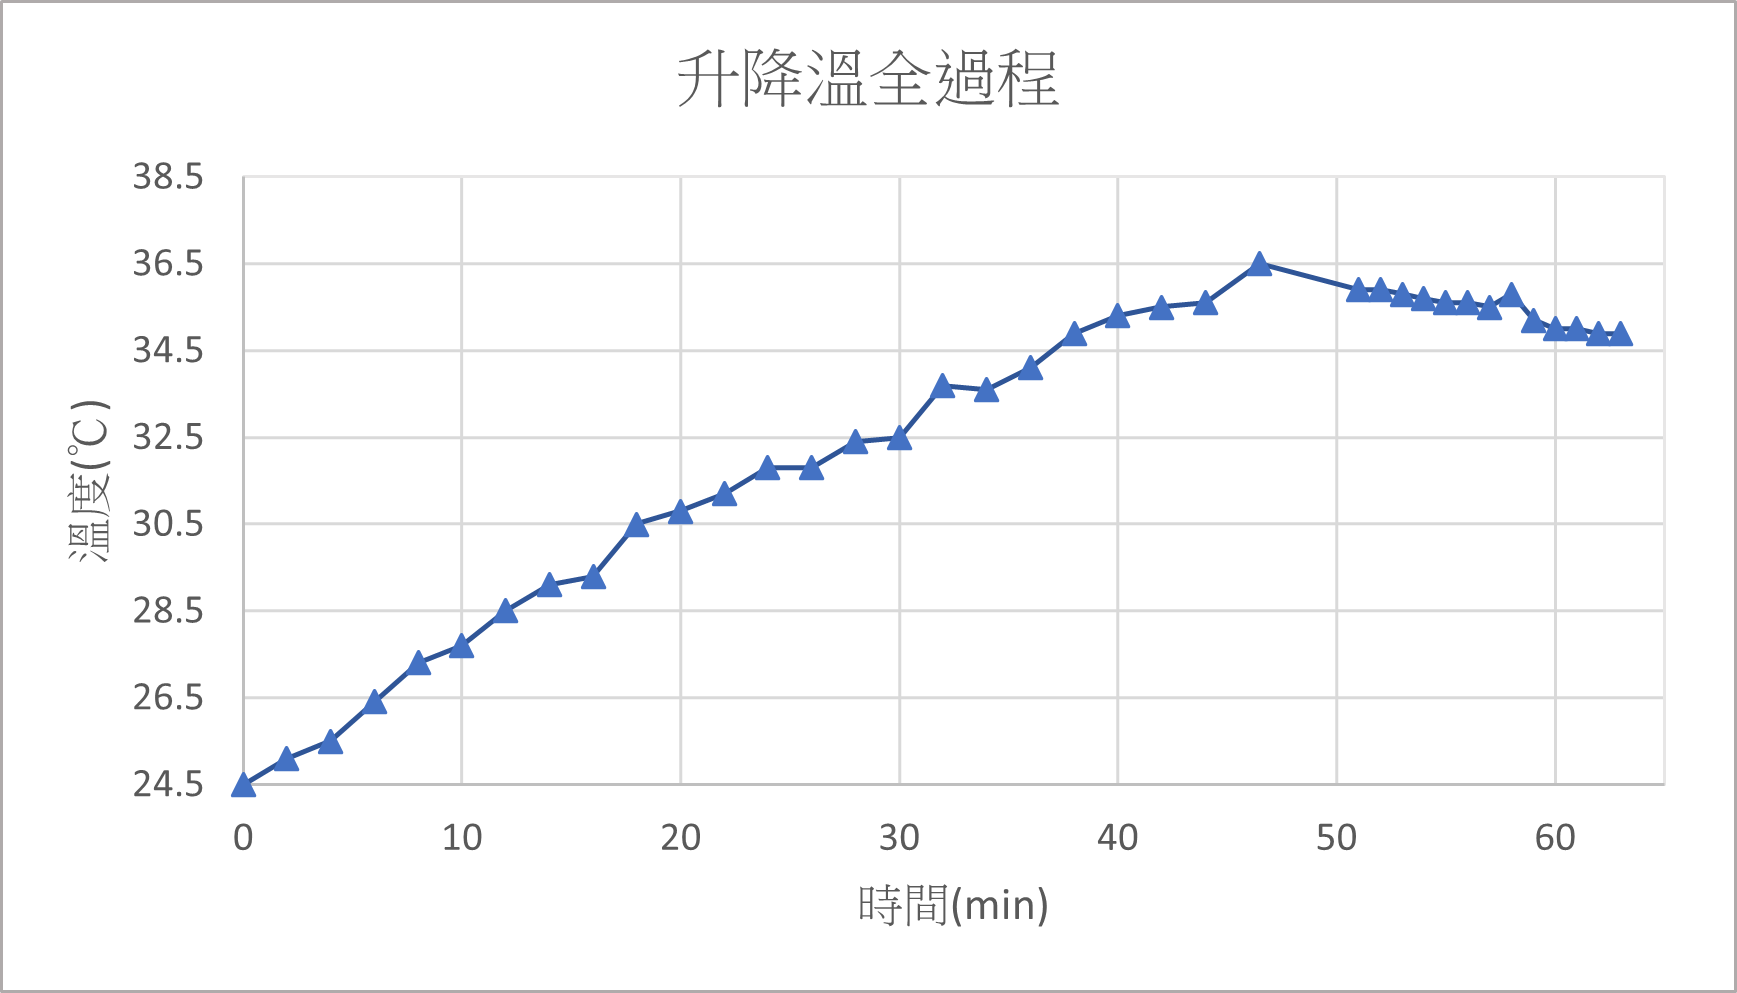
\includegraphics[width=0.5\linewidth]{熱功當量/熱功當量/圖表/升降溫.png}
     \caption{時間t與溫度T的關係圖}
     \label{fig:時間t與溫度T的關係圖}
     \end{figure}
     \item 加熱總時間:$t_f=46.5(\text{min})$，$t_f$時刻量得的系統溫度$T_f=36.5(^\circ \text{C})$，\\停止加熱時間$t_R=16.5(\text{min})$，$t_R$時刻量得的系統溫度$T_R=34.9(^\circ \text{C})$，\\$\kappa=\frac{1}{t_R-t_f}\ln(\frac{T_R-\theta}{T_f-\theta})\approx -0.0055$，
     散熱導致的溫差$\Delta T=1.17^\circ \text{C}$;\\
     修正後的末溫$T_H=T_ f+\Delta T=36.5^\circ \text{C} + 1.17^\circ \text{C} = 37.67^\circ \text{C}$;\\
     \item 外界提供的總電能：
    總加熱時間 $t_f = 46.5 \text{ min} = 2790 \text{ s}$。
     \[
     W = V \cdot I \cdot t_f = 9.99 \text{ V} \cdot 0.617 \text{ A} \cdot 2790 \text{ s} \approx 17197.09 \text{ J}
    \]
    
     \item 系統吸收的總熱能 $Q$ 的計算（假設系統總熱容量 $C_{total} = 290.98 \frac{\text{cal}}{^\circ \text{C}}$）：\\
     修正後的溫升 $\Delta T_{correct} = T_H - T_0 = 37.67^\circ \text{C} - 24.5^\circ \text{C} = 13.17^\circ \text{C}$。
     \[
     Q = C_{total} \cdot \Delta T_{correct} = 290.98 \frac{\text{cal}}{^\circ \text{C}} \cdot 13.17^\circ \text{C} \approx 3833.09 \text{ cal}
     \]
    
     \item 熱功當量 $J$ 的計算：
    \[
     J = \frac{W}{Q} = \frac{17197.09 \text{ J}}{3833.09 \text{ cal}} \approx 4.487 \text{J}/\text{cal}
    \]
    
     \item 誤差分析：
     相較於公認值 $4.186 \text{J}/\text{cal}$，本次實驗結果的誤差約為 $7.19\%$。
    \end{itemize}
%%%%%%%%%%%%%%%%%%%%%%%%%%%%%%%%%%%%%%%%%%%%%%%%

\subsection{\textbf{誤差分析 (Discussion on Errors)}}

根據實驗結果，測得的熱功當量 $J \approx 4.487 \text{J}/\text{cal}$ 與公認值 $4.186 \text{J}/\text{cal}$ 相比，誤差約為 $\mathbf{7.19\%}$。由於實驗值 $J$ 偏高，根據 $J = W/Q$ 的關係，這意味著系統吸收的有效熱能 $Q$ 被低估，或輸入電能 $W$ 被高估。以下是推測的誤差來源。
\subsubsection{系統性誤差}

系統性誤差是導致 $J$ 值偏高的主要原因，尤其與熱容量測定和散熱修正的準確性有關。

\begin{table}[H]
    \centering
    \caption{系統性誤差分析}
    \begin{tabular}{p{4cm} p{5cm} p{4cm}}
        \toprule
        \textbf{來源} & \textbf{影響機制} & \textbf{最終影響} \\
        \midrule
        \textbf{卡計熱容 $C$ 測定不準確} & 實驗一混合法中，高溫水在混合前或混合過程中散失熱量，導致平衡溫度 $T_{ave}$ 偏低，計算所得的卡計水質量 $m$ 偏小。 & $C$ 偏小 $\rightarrow Q$ 低估 $\rightarrow J$ 偏高 \\
        \midrule
        \textbf{電錶校準問題} & 若用於測量電壓 $V$ 或電流 $I$ 的電錶讀數存在系統性偏高，則導致計算所得的總電能 $W = V I t$ 被高估。 & $W$ 高估 $\rightarrow J$ 偏高 \\
        \midrule
        \textbf{溫度計延遲/位置} & 溫度計的反應速度慢，未能及時捕捉到系統的實際最高溫 $T_f$，或溫度計未放置在水的平均溫度處。 & $\Delta T$ 偏小 $\rightarrow Q$ 低估 $\rightarrow J$ 偏高 \\
        \bottomrule
    \end{tabular}
\end{table}

\subsubsection{散熱修正的不足 }

散熱修正是本實驗精確性的關鍵。使用的單一 $\kappa$ 值模型未能完全模擬真實的熱傳遞過程。

\begin{itemize}
    \item \textbf{冷卻係數非定值 $\kappa$}：
    散熱係數 $\kappa$ 是通過降溫過程的數據計算得到的，但此計算假設 $\kappa$ 在整個升溫過程中保持不變。在加熱過程中，系統溫度較高，熱輻射的影響（正比於絕對溫度的四次方 $T^4$）會更為顯著，導致實際 $\kappa$ 隨溫度升高而略微增加。採用單一 $\kappa$ 值會**低估**高溫階段的散熱量。
    \item \textbf{修正方法近似}：
    無論是使用積分近似法或平均溫差法來計算總修正量 $\Delta T_{loss} = 1.17^\circ \text{C}$，都是基於牛頓冷卻定律的近似。如果升溫過程的溫度變化是非線性的，會導致修正量本身不夠精確，從而使得修正後的末溫 $T_H$ 仍有偏差。
\end{itemize}

\subsubsection{隨機誤差}
\begin{itemize}
    \item \textbf{計時與同步誤差：} 在啟動/停止電源與碼錶計時之間不同步，會影響總加熱時間 $t_f$ 的精確度。
\end{itemize}

%%%%%%%%%%%%%%%%%%%%%%%%%%%%%%%%%%%%%%%%%%%%%%%%%%%%%%%%%%%%%%%%
\newpage
\section{\textbf{結果與討論}}
In this experiment, the\textbf{ mechanical equivalent of heat }was determined by combining \textit{calorimetric} measurements with \textit{electrical energy} input, under the assumption of energy conservation. The system heat capacity was first obtained using the \textbf{method of mixtures,} and the electrical work supplied during heating was calculated from\textit{\textbf{ measured voltage, current, and heating time.}} To improve accuracy, a heat-loss correction was applied using the cooling curve and Newton’s law of cooling.

\vspace{0.3cm}
After applying the \textbf{heat-loss correction}, the corrected final temperature of the system was $T_H=37.67\ ^∘C$, corresponding to a corrected temperature rise of $\Delta T_{correct}=13.17\ ^ \circ C$ .Using a total system heat capacity of $C_{total}=290.98\  cal/^\circ C \,$ the absorbed thermal energy was calculated to be $Q\approx3833.09\ cal.$ The total electrical energy supplied was $ W\approx1.72×104\ J$, leading to an experimentally determined \textit{mechanical equivalent of heat,}
\vspace{0.3cm}
\[J=\frac{W}{Q}\approx 4.487\ J/cal.\]

\vspace{0.3cm}
This result is \textbf{higher} than the accepted value of $4.186 \ J/cal$ by approximately 7.19\%. Since $ J=W/Q$, a higher experimental value suggests that the\textit{ absorbed heat} \textit{Q} was \textbf{underestimated} or that the supplied \textit{electrical energy W} was \textbf{overestimated}. Several factors likely contributed to this deviation. Systematic errors, such as an underestimated calorimeter heat capacity due to \textbf{heat loss} during the mixing process, would reduce the calculated $Q$. In addition, limitations in electrical measurement accuracy could lead to a \textbf{slight overestimation} of $W$. Temperature measurement effects, including thermometer response delay and non-uniform temperature distribution within the water, may also have caused the measured temperature rise to be smaller than the true average value. 

\vspace{0.3cm}
The heat-loss correction, while necessary, introduces further approximation. The cooling coefficient $\kappa$ was determined from the\textbf{ post-heating cooling curve} under the assumption that it remains \textbf{constant} throughout the heating process. In reality, heat transfer mechanisms become \textit{more significant at higher temperatures}, and the use of a single $\kappa$ value may not fully account for heat loss during the \textbf{later stages of heating}. Consequently, the corrected temperature rise may still be slightly underestimated, contributing to the observed overestimation of $J$. 

\vspace{0.3cm}
Despite these limitations, the experimental data show a clear and consistent relationship between \textbf{electrical work} and\textbf{ thermal energy increase.} The \textit{magnitude} of the measured heat equivalent is reasonably close to the accepted value, and the observed error lies within an expected range for a calorimetry experiment with unavoidable heat exchange. Therefore, while the numerical accuracy is limited, the experiment can be considered an \textbf{overall success} in verifying the\textit{ principle of energy conservation} and demonstrating the practical challenges of precise heat measurements.

 
\newpagea
\section{\textbf{思考問題}}

\hrule
\vspace*{0.5cm}
%%%%%%%%%%%%%%%%%%%%%%%%%%%%%%%%%%%%%%%%%%%%%%%%%%%%%%%%%%%%%
\noindent
\textbf{$Q_1:T_0$是否一定要是在系統加熱前的溫度?可否任意選定?是否加熱一開始即須計時?}
\begin{itemize}
    \item $T_0$ 在定義中是加入銅杯內水的溫度，並未與卡計熱平衡，因此$T_0$可以選用與卡計熱平衡後的溫度。
    \item 不可任意選定，因為$T_0$影響卡計熱容的計算。
    \item 是。因為計算熱功當量計算是以外界提供的電能來換算，所以不可任意更改時間，該行為會造成電能計算不精確。
\end{itemize}
%%%%%%%%%%%%%%%%%%%%%%%%%%%%%%%%%%%%%%%%%%%
\vspace*{0.5cm}
\noindent
\textbf{$Q_2:$以實驗數據說明散熱修正的必要性。並討論不進行修正會造成多大的誤差?\\}
\begin{itemize}
    \item 在實驗過程中，即使停止加熱，水溫也會逐漸下降（即降溫過程或冷卻曲線）。這段降溫本身就是系統持續向環境散熱的直接證據。故此修正的必要性可顯。
    \item 下表是修正散熱與不修正的比較:
    \begin{table}[H]
    \centering
    \begin{tabular}{cccc}
    \hline
         & $T$   & $T+\Delta T$               &                                    \\ \hline
    溫度   & 36.50 & 37.67                      &                                    \\ \hline
    熱功當量 & 4.486 & 4.544                      &                                    \\ \cline{4-4} 
    誤差   & 7.2\% & \multicolumn{1}{l|}{8.6\%} & \multicolumn{1}{l|}{熱功當量準確值:4.186} \\ \hline
    \end{tabular}
    \end{table}
    有此可得出，在不進行修正的前提，所測得的熱功當量相比修正後有更大的誤差$(7.2\% \rightarrow8.6\%) $
\end{itemize}

%%%%%%%%%%%%%%%%%%%%%%%%%%%%%%%%%%%%%%%%%%%
\vspace*{0.5cm}
\noindent
\textbf{$Q_3:$如何判定散熱修正後，末溫是正確的?}
\begin{itemize}
    \item 如果修正後的熱功當量 $J$ 值與公認值（$4.186 \text{ J/cal}$）非常接近（誤差小於 $5\%$），則可以推斷修正後的末溫 $T_{f\_correct}$ 是正確的。
\end{itemize}
%%%%%%%%%%%%%%%%%%%%%%%%%%%%%%%%%%%%%%%%%%%
\vspace*{0.5cm}
\noindent
\textbf{$Q_4:$分別利用以下兩式所得的溫差$\Delta T$相差多少?}
\begin{center}
    方法一: $dT=\int_{t}^{t+\Delta t}\kappa\cdot(T-\theta)\,dt\approx \Delta t \cdot [\kappa\cdot(T-\theta)]$\\\\
    
    方法二: $\vert\Delta T=  \kappa\cdot(\frac{T_f+T_0}{2}-\theta) \vert$
\end{center}
\begin{enumerate}
    \item 首先，使用excel列出每一段時間間隔的平均溫來計算$dT$。
    \item 結果如下表:
    \begin{table}[H]
    \centering
    \begin{tabular}{cccc}
    \hline
    修正方法 & 方法一 & 方法二               &                                    \\ \hline
    溫度   & 37.79 & 37.67                      &                                    \\ \hline
    熱功當量 & 4.446 & 4.544                      &                                    \\ \cline{4-4} 
    誤差   & 6.2\% & \multicolumn{1}{l|}{8.6\%} & \multicolumn{1}{l|}{熱功當量準確值:4.186} \\ \hline
    \end{tabular}
    \end{table}
    可見方法一相比方法二準確度更高
\end{enumerate}
%%%%%%%%%%%%%%%%%%%%%%%%%%%%%%%%%%%%%%%%%%%
\vspace*{0.5cm}
\noindent
\textbf{$Q_5:\kappa$值是否與溫度有關?}
\begin{itemize}
    \item 是。散熱係數 $\kappa$ 包含了所有熱傳遞的貢獻：傳導、對流和輻射。
    \item 傳導和對流： 這兩種模式的熱傳遞係數對溫度有依賴性，但通常在實驗所涉及的溫差範圍內（幾十攝氏度）變化不大。
    \item 輻射： 根據史蒂芬-波茲曼定律，輻射的散熱功率正比於 $T^4$。這表示輻射散熱對溫度非常敏感。當實驗溫度較高時（例如超過 $50^\circ \text{C}$），輻射的影響會變得很顯著，此時 $\kappa$ 就會明顯隨溫度升高而增大。

\end{itemize}

\vspace*{0.5cm}
\hrule
\vspace*{0.5cm}
\end{document}